\documentclass[pageno]{jpaper}
%\newcommand{\iscasubmissionnumber}{117}

\usepackage[normalem]{ulem}
\usepackage{booktabs}
\usepackage{mathtools}
\usepackage{ragged2e}
\usepackage{rotating}
\usepackage{array}
\usepackage{grffile}

\usepackage{epsfig}
\usepackage{float}
\usepackage{wrapfig}
\usepackage{setspace}
\usepackage{multirow}
\usepackage{graphicx}
\usepackage{fancyhdr}
%\usepackage{paralist}
%\usepackage{capt-of}

\usepackage{color}
\usepackage{xcolor,colortbl}
\usepackage{chngpage}
\usepackage{enumitem}
\usepackage{enumerate}
\usepackage{amsmath,relsize}
\usepackage[justification=centering]{caption}
\usepackage{tabu}
\usepackage{stmaryrd} % short right arrow

\usepackage{listings}
\usepackage[makeroom]{cancel}


\usepackage{amssymb}% http://ctan.org/pkg/amssymb
\usepackage{pifont}% http://ctan.org/pkg/pifont
\usepackage[nomargin,inline,draft]{fixme}
\newcommand{\cm} {\clap{\small\ding{51}}\small\hphantom{--}}
\newcommand{\cmi}{\clap{\small\ding{51}-}\small\hphantom{--}}%
%\newcommand{\xm} {\clap{\ding{55}}\hphantom{--}}
\newcommand{\xm} {\clap{\small}\small\hphantom{--}}

\newcommand{\Forall}{\displaystyle\mathop\mathlarger{\mathlarger{\mathlarger{\forall}}} } 

%\newcommand{\cm} {{Y}}%
%\newcommand{\cmi}{{P}}%
%\newcommand{\xm} {{}}%


\usepackage{tikz,array}
\usetikzlibrary{calc}

%\newcommand*\circled[1]{\tikz[baseline=(char.base)]{
%            \node[shape=circle,draw,inner sep=2pt] (char) {#1};}}

%\newcommand*\ccircled[1]{\tikz[baseline=(char.base)]{
%            \node[shape=circle,draw,inner sep=2pt] (char) {#1};}}

\tikzstyle{every node}=[font=\footnotesize]

\newcommand{\hcancel}[5]{%
    \tikz[baseline=(tocancel.base)]{
        \node[inner sep=0pt,outer sep=0pt] (tocancel) {#1};
        \draw[black] ($(tocancel.south west)+(#2,#3)$) -- ($(tocancel.north east)+(#4,#5)$);
    }%
}%

\newcommand*\circled[1]{\tikz[baseline=(char.base)]{
            \node[shape=circle,draw,inner sep=0.5pt, minimum size=0.24cm] (char) {#1\vphantom{H}};}}

\newcommand*\ccircled[1]{\hcancel{\tikz[baseline=(char.base)]{
            \node[shape=circle,draw,inner sep=0.4pt, minimum size=0.24cm] (char) {#1\vphantom{H}};}}{-1pt}{1pt}{1pt}{-1pt} }


\begin{document}
\title{
\vspace{-0.15in}
An Efficient GPGPU Implementation of Viola-Jones Classifier Based Face Detection Algorithm
\vspace{-0.15in}
}





\author{Sharmila Shridhar  \\ \and 
				Vinay Gangadhar  \\ \and  
				Ramsai Manoj Bamdhamravuri   \\ \and
            \{gangadhar, sshridhar, ranganagoudr\}@wisc.edu} 

%\author{Vinay Gangadhar \\ vinay@cs.wisc.edu \\ \and 
%				Sharmila Shridhar \\ sshridhar@wisc.edu \\ \and  
%				Anil Ranganagoudra  \\ ranganagoudr@wisc.edu \\ \and
%				Chandana Hosamane 	\\ hosamane@wisc.edu} 

\date{}
\maketitle

%\thispagestyle{empty}
\begin{abstract}
   
\vspace{0.1in}

Applications with large amount of data level parallelism
can benefit from General Purpose based Graphics Processing
Units (GPGPUs) because of better energy efficiency and performance compared to a CPU. Due to GPGPUs’ impressive
computing throughput and memory bandwidth, many applications with enough parallelism can take advantage of acceleration using GPGPU. Computer vision algorithms are one such
workload domain which can better utilize the large number
of cores in GPU, and hence meet their real-time requirements
of the applications. One such application is \emph{Face Detection}
which has real-time constraint on its execution. Sequential
processing of image windows with image downsampling and classifiers on CPU is difficult to meet the real-time requirements. 

In this project, we have
implemented the face detection acceleration algorithm based
on Viola-Jones cascade classifier on the GPGPU CUDA platform.
We have considered different portions of the viola jones algorithm which include 
\emph{nearest neighbor}, \emph{integral image} and {HAAR classifier} that can
be parallelized.
We identify different bottlenecks in GPU implementation and include optimizations
which gives the performance benefit. We explain each of these optimizations in detail for all the kernels. 
We finally compare the execution of the same algorithm executed
on the CPU and analyze the gains from the GPU.
We achieve a speedup upto 5.35x (including the inclusive time) compared to the single threaded performance of CPU.




\end{abstract}

\section{Motivation}\label{sec:motivation}


In this project, we intend to implement face detection algorithm based on the Viola Jones classifier \fixme{ref} on GPU. 
As a starting point, we take the GNU licensed C++ program that has the 
algorithm implemented to detect faces in images \fixme{ref}. 
There are various portions in the algorithm that can be parallelized and hence can leverage the hardware of GPU efficiently. 
Section 1 explains Viola Jones algorithm briefly. Section 2 explains the portions we are going to parallelize and offload to the GPU.


Viola Jones Face Detection Algorithm
The algorithm has four stages:
Haar feature selection: The Viola Jones classifier method is based on Haar-like features. 
The features consist of white and black rectangles as shown in Fig 1. 
These features can be thought of as pixel intensity evaluation sets. 
For each feature, we subtract black region’s pixel value sum from white region’s pixel value sum. 
If this sum is greater than some threshold, it is decided that the region has this feature. 
This is the characteristic value of a feature. We have the Haar features
to be used for face detection

 
\section{Background and Proposed PENN Architecture}\label{sec:arch}

Before explaining the high level organization of PENN
architecture, we define the five specialization principles 
we employed to consider this style of architecture.
Our primary insight on coming to the architectural substrate
is based on well-understood mechanisms of specialization used in DSAs.
We first explain the assumptions we make for neural network workloads based on
our preliminary analysis.

\paragraph{Workload Assumptions}
1. Neural network workloads have significant parallelism, 
either at the data or thread level. 2. They perform some problem specific complex 
computational work and not just data-structure traversals. 3. They have coarse grain units of work. 
4. They have regular memory access patterns.

\subsection{Specialization Principles}

Broadly, we see these principles as a counterpart to the insights from Hameed et
al.~\cite{gpp_innef}, in that they describe the sources of inefficiency in a
general purpose processor, whereas our findings are oriented around
elucidating the sources of potential efficiency gain from specialization.  

\paragraph{Concurrency Specialization}
The concurrency of a workload is the degree to which its operations can be performed
in parallel. This concurrency can be derived from data or thread level parallelism
found in the workloads. 
Examples of specialization strategies
include employing many independent processing elements with their own controllers,
or using a wide vector model with a single controller.
We chose the former one as baseline architecture having many processing elements
with a low-power controller.

\paragraph{Computation Specialization}  
Computations are individual units of work in an algorithm executed by
functional units (FUs).
Specializing \emph{computation} means creating problem-specific FUs.  
For instance, a \texttt{sin} FU would much more efficiently compute the sine function than
iterative methods on a general purpose processor.
Specializing computation improves performance and energy by
reducing the total work.
Most of the neural network applications employ some commonality
in FU types.

\paragraph{Communication Specialization} 
Communication is the means of transmission of transient
values between the storage and functional units.  Specialized
communication is simply the instantiation of communication channels, and
potentially buffering, between FUs to ultimately facilitate a faster
operand throughput to the FUs.  This reduces power by lessening access
to intermediate storage, and potentially area if the alternative is a general
communication network.  

\paragraph{Data Reuse Specialization} 
Data reuse is an algorithmic property where intermediate
computed values are consumed multiple times.  
The specialization of data reuse means using
custom storage structures or reuse buffers for these temporaries.
Specializing reuse benefits performance and power by avoiding 
the more expensive access to a larger global memory or register files.

\paragraph{Coordination Specialization} 
Hardware coordination is the management of multiple hardware
units and their timing to perform  work.  Instruction
sequencing, control flow, interrupts handling and address generation are all
examples of coordination tasks.  
Specializing it usually involves the
creation of small finite state machines to perform each task.
A low-power in-order core or a micro-controller could be used for this coordination specialization.

\subsection{PENN Architecture}

\begin{figure}
  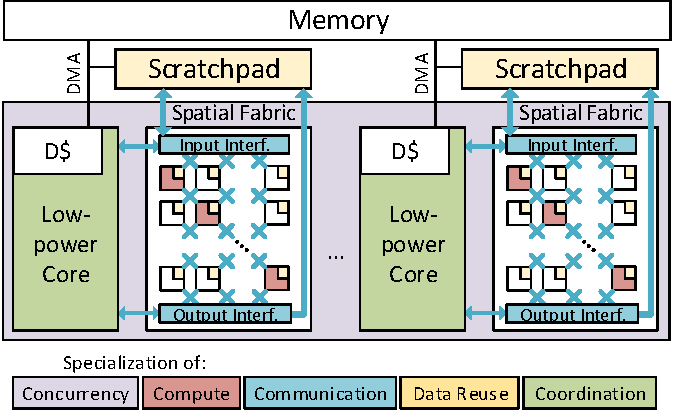
\includegraphics[width=\linewidth]{figs/fabric_5p.pdf}
  \vspace{-0.1in}
  \caption{Programmable Engine for Neural Networks (PENN) Architecture \textnormal{\small }  }
  \label{fig:penn-fabric}
\end{figure}

Figure~\ref{fig:penn-fabric} gives a high level overview of the PENN architecture 
we have proposed. 
The requirement to exploit high concurrency in workloads pushes the design towards simplicity, 
and the requirement of programmability implies the use of some sort of programmable core.
The natural way to fill these combined requirements is to use an array of tiny
low-power cores which communicate through memory.
These low power cores have caches, general purpose programmable and
are basic building blocks of PENN. The low-power core along with
other specialization units (explained below) form one unit of PENN fabric and
multiple such units are used to specialize \emph{Concurrency}.
Using many units, as opposed to a wide-vector model, has a flexibility advantage.  When
memory locality is not possible, parallelism can still be achieved through
multiple execution threads.  The remainder of the design is to straight-forwardly
apply the remaining specialization principles.

Achieving \emph{communication} specialization of intermediate values requires
an efficient distribution mechanism for operands, which avoids expensive
intermediate storage like multi-ported register files.  Arguably, the best
known way to do this is to use an explicit routing network, which is exposed to
the ISA to eliminate the hardware burden of dynamic routing.  This property is
what defines spatial architectures and therefore we add a spatial
architecture as our first mechanism. The spatial architecture 
can be a Coarse Grain Reconfigurable Fabric (CGRA) which has an
intermix of FUs connected spatially through an interconnected network. 
This serves two additional purposes.
First, it is an appropriate place to instantiate custom functional units, i.e.
\emph{computation} specialization.  Second, it accommodates \emph{reuse} of
constant values associated with specific computations.  In principle, this
spatial architecture can be either fine-grain reconfigurable (FPGA) or more
coarse grain reconfigurable.

To achieve \emph{communication} specialization with the global memory, a natural
solution is to add a DMA engine and configurable scratchpad, with a vector
interface to the spatial architecture.  The scratchpad, configured as a DMA
buffer, enables the efficient streaming of memory by decoupling memory access from the
spatial architecture.  When configured differently, the scratchpad can act as a
\emph{reuse} buffer.  In either context, a single-ported scratchpad is
enough, as access patterns are usually simple and known ahead of time.

Finally, we require an efficient mechanism for \emph{coordinating} the above
hardware units (e.g. configuring the spatial architecture or
synchronizing DMA with the computation).  Again, here we propose relying on the
simple core, as this brings a huge programmability and generality benefit.
Furthermore, the cost is low; if the core is low-power enough, and the spatial 
architecture is large enough, the overheads of coordination can be kept low.

To summarize, each unit of our proposed architecture contains a Low-power core,
a Spatial architecture, Scratchpad and DMA.
This architecture satisfies the programmable accelerator requirements:
general-purpose programmability, efficiency through the application of
specialization principles, and simple parameterizability.


\paragraph{PENN in Practice}

Preparing the PENN for use occurs in two phases: 
1. \emph{design synthesis} -- the selection of hardware parameters to suit the chosen workload
domain; and 2. \emph{programming} -- the generation of the program and spatial
datapath configuration to carry out the algorithm.

For our project, though many optimization strategies are possible, 
we  want to consider the 
primary constraint of this programmable architecture to be performance -- i.e. there
exists some throughput target that must be met, and power and area should be
minimized, while still retaining some degree of generality and programmability. 
We want to explore micro-architectural design decisions needed to make this
design synthesis step easier and efficient for many workload kernels.

Programming PENN has two major components: creation of the coordination
code for the low power core and generation of the configuration data/stream for the
spatial datapath to match available resources.  
In practice using standard languages with
\texttt{\#pragma} annotations, or even languages like OpenCL would likely be more
effective.  
Though we do not aim to implement a full-working compiler in this project,
we want to develop an API for PENN programming and hand-generate assembly instructions
along with configuration stream to configure PENN.
Figure~\ref{fig:ex-prog} shows an example annotated code for computing 
a neural network layer, along with a provisioned (already synthesized) PENN.  
The figure also shows the compilation steps to map each portion of the code to the 
architecture.  At a high level, the compiler will use annotations to identify
arrays for use in the SRAM, and how should they be used (either as a stream buffer or scratchpad). 
In the example, the weights can be loaded into the scratchpad, and reused across
invocations.
 
Subsequently, the compiler will unroll and create a large-enough datapath to
match the resources present in the spatial fabric, which could be spatially
scheduled using scheduling techniques. Communication
instructions would be inserted into the coordination code, as well as
instructions to control the DMA access for streaming inputs.  Finally, the
coordination loop would be modulo scheduled to effectively pipeline the spatial
architecture.

\begin{figure}
  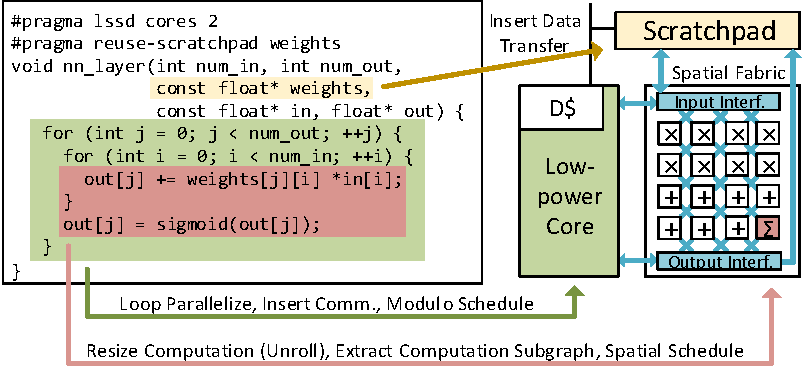
\includegraphics[width=\linewidth]{figs/example_prog.pdf}
  \vspace{-0.1in}
  \caption{Example Program \& Compiler Passes \newline
  \textnormal{\small (Arrows labeled with required compilation passes.)} 
}
  \label{fig:ex-prog}
\end{figure}


\section{Project phases}\label{sec:plan}

We explain the phases of project here and expected timeline for 
each step. Some of the phases can be carried out in parallel and will be distributed 
among the project members.

\begin{itemize}
\item \textbf{Phase 0 [1 week]:} Choose the representative workloads/ kernels of neural network domain
targeting different applications (image processing, speech recognition, text parsing etc.,). 
Use the trace based modeling tool TDG (~\cite{tonytdg}) modeled
for PENN to determine the initial performance and power estimates for each kernel.
More accurate analysis of workloads (profiling) to be done here and see if there are any missing architectural
pieces not considered for current PENN architecture.

\item \textbf{Phase 1 [2 days]:} Based on phase 0 analysis, some important design trade-off decisions should be taken. Those steps are listed here:
i) Low-power core: Properties (pipeline stages, memory interface and hierarchy etc.,) of low-power core which does the co-ordination.
Compiler and software toolchain for the core (RISCV toolchain and their in-order core can be a good start). 
ii) CGRA: Types of problem specific FUs inside the fabric.  Interface to low-power core and scratchpad memory.
Addressing of scratchpad space and global memory. Scheduling pattern for CGRA. Scratchpad size and bit-width.
iii) Programming model: API for PENN. Pragmas and code annotations for compilation.

\item \textbf{Phase 2 [3 weeks]:} This phase involves implementation of individual modules of PENN listed in Phase 1. 
Implementation of low power core and CGRA in Verilog and C++.
Writing API routines for PENN and compiler support (Note: A full-fledged compiler may not be implemented but 
a framework to generate instructions and configuration stream will be implemented.)
Tools needed for the project are explained in Section~\ref{sec:meth}.

\item \textbf{Phase 3 [1 week]:}This phase mainly involves evaluating implemented synthesized PENN architecture with
    representative workloads chosen in Phase 0. We also use C++ simulator written for PENN to correlate the functionality of the synthesized version. 
We plan to evaluate PENN for performance, area and power against a state-of-the-art DSA for Neural Network.

\item \textbf{Phase 4 [2 weeks]:} This phase mainly involves prototyping PENN on Zynq FPGA. However, this phase will be realized only if Phase 3 is
    completed well within course project time limit. Project report is also part of this phase.
\end{itemize}




 
\section{Methodology }\label{sec:meth}
<<<<<<< HEAD

=======
We try to list out some of the tools we are considering for our project and also the methodologies involved with those.

We plan to use existing RISCV LLVM toochain~\cite{nguyenlinux} as part of compiler framework. 
For low power core, we are considering a three stage pipeline SODOR core as it is power efficient compared to any standard VLIW core. 
For implementing individual modules, we want to use CHISEL~\cite{chisel2012} tool, which uses an embedded scala language to generate verilog code and C++ simulator
framework. Also, for our initial modeling phase, we used a trace based modeling tool TDG and we will be using the same for our further analysis.   

For evaluating PENN, we will be collecting performance, power and area statistics of the synthesized version and compare it with statistics 
given in the literature of DSA papers. 
>>>>>>> 49ddcfc99c241d091550ef080d974a6076980d94

\section{Related Work}\label{sec:related}


%\input{architecture}
%\input{compiler}
%\input{methodology}

\bstctlcite{bstctl:etal, bstctl:nodash, bstctl:simpurl}
\bibliographystyle{IEEEtranS}
\bibliography{main}

\end{document}
